\rhead{\small \textcolor{sugray}{Name: \hskip2.8cm}}
\rightline{\raise 10pt\hbox{\small \textcolor{sugray}%
{Final, 3:30--6:30\,pm, December 13, 2017}}}

\problem8
Consider a homogeneous thermodynamic system 
of $N$ particles confined inside 
a volume $V$ being held at temperature $T$.
Each particle occupies a constant volume $v_0$.
Let $T_0 = 300\,{\rm K}$ denote a reference temperature.
Assume that the system is at stable equilibrium.

\medskip \noindent
Which of the following expressions is a plausible candidate for the system entropy?
State your reasoning for accepting or rejecting each of the four options.
Two points will be granted for each correct answer.
\begin{align*}
&\text{(a) }  S = \frac{\kB\, T}{N\, T_0} + \kB \exp\left(\frac{V}{v_0}\right)
&\text{(b) }& S = \frac{N\kB T_0}{T} + N\kB \ln\left(\frac{V}{N v_0}\right)\\
&\text{(c) }  S = N \kB \ln\left(\frac{T}{T_0}\right) + \kB \frac{(V/v_0)^2}{N}
&\text{(d) }& S = N \kB \ln\left(\frac{V\, T}{N v_0\, T_0}\right)
 \end{align*}
\solution{\\
There are three constraints: 
(1) entropy must be extensive, 
(2) $\pdc{^2 S}{V^2}{N,T} \leq 0$, and
(3) $\pdc{^2 S}{N^2}{V,T} \leq 0$.
Conditions (2) and (3) are required for equilibrium 
(system is thermodynamically stable).
There are two conditions because $S(N,V,T)$ has explicit
dependence on two extensive variables, $V$ and $N$.
\begin{enumerate}
\item \boxed{\text{Invalid.}} 
\[ S (\lambda N, \lambda V, T) 
   = \frac{\kT}{\lambda N T_0} + \kB \exp \left( \frac{\lambda V}{v_0} \right) 
\neq \lambda S(N,V,T) \]
Condition (1) is violated because entropy is not extensive.
%
%
\item \boxed{\text{Valid!}}
\begin{align*}
  S (\lambda N, \lambda V, T) 
   &= \frac{\lambda N \kT}{T} 
    + \lambda N \kB \ln \left( \frac{\lambda V}{\lambda N v_0} \right) 
    = \lambda S(N,V,T) \\
 \pdc{^2 S}{V^2}{N,T} 
   &= \frac{\partial}{\partial V} \left[ 0 + \frac{N \kB}{V} \right]_{N,T} 
    = \frac{-N k_B}{V^2} < 0 \\
 \pdc{^2 S}{N^2}{V,T} 
   &= \frac{\partial}{\partial N} \left[ \frac{\kB T_0}{T} 
    + \kB \ln \left( \frac{V}{v_0} \right) 
    - \kB (1 + \ln N ) \right]_{V,T} 
    = 0 + 0 - \frac{\kB}{N} < 0
\end{align*}
All of our constraints are satisfied, so this is a plausible entropy expression.
%
%
\item \boxed{\text{Invalid.}}
\[ \pdc{^2 S}{V^2}{N,T} 
 = \frac{\partial}{\partial V} \left[ 0 + \frac{\kB}{N v_0^2} (2 V) \right]_{N,T} 
 = \frac{2 \kB}{N v_0^2} (1) > 0 \]
Condition (2) is violated because the curvature of $S$ with respect to $V$ is positive.
%
%
\item \boxed{\text{Valid!}}
\begin{align*}
  S (\lambda N, \lambda V, T) 
   &= \lambda N \kB \ln \left( \frac{\lambda V T}{\lambda N v_0 T_0} \right) 
    = \lambda S(N,V,T) \\
 \pdc{^2 S}{V^2}{N,T} 
   &= \frac{\partial}{\partial V} \left[ \frac{N \kB}{V} \right]_{N,T} 
    = \frac{-N \kB}{V^2} < 0 \\
 \pdc{^2 S}{N^2}{V,T} 
   &= \frac{\partial}{\partial N} \left[ 
      \kB \ln \left( \frac{V T}{v_0 T_0} \right) 
    - \kB (1 + \ln N) \right]_{V,T} 
    = 0 - \frac{\kB}{N} < 0
\end{align*}
All of our constraints are satisfied, so this is a plausible entropy expression.
\end{enumerate}
\newpage
}


\problem8
The mixing free energy of a binary incompressible blend
can be written as
\[ F(x, T) = (n_1 + n_2) f(x, T) .\]
Here $n_1$ and $n_2$ are molecular numbers,
$x \equiv n_1 / (n_1 + n_2)$ is the mole fraction of species~1,
and $f(x, T)$ is defined as the free energy per molecule.

\smallskip \subp
Show that the chemical potentials $\mu_1$ and $\mu_2$
satisfy the following Gibbs-Duhem relation:
\[ x \left. \frac{\partial \mu_1}{\partial x} \right|_T 
+ (1 - x) \left. \frac{\partial \mu_2}{\partial x} \right|_T = 0.
\]
\solution{
Assuming $T$ is constant, let $f'(x,T) \equiv \pdc{f}{x}{T}$ and
$f''(x,T) \equiv \pdc{^2 f}{x^2}{T}$.
\begin{align*}
   \mu_1 \equiv \pdc{F}{n_1}{n_2,T} 
      &= (n_1 + n_2) \pdc{f}{n_1}{n_2,T} 
       + f \pdc{(n_1 + n_2)}{n_1}{n_2,T} \\
      &= (n_1 + n_2) \pdc{f}{x}{n_2,T} \pdc{x}{n_1}{n_2,T} + f \\
      &= (n_1 + n_2) (f') 
         \left( \frac{(n_1 + n_2) - n_1}{(n_1 + n_2)^2} \right) + f \\
      &= f' \left( \frac{n_2}{n_1 + n_2} \right) + f \\
      &= (1-x) f' + f
\end{align*}
\begin{align*}
   \mu_2 \equiv \pdc{F}{n_2}{n_1,T} 
      &= (n_1 + n_2) \pdc{f}{n_2}{n_1,T} 
       + f \pdc{(n_1 + n_2)}{n_2}{n_1,T} \\
      &= (n_1 + n_2) \pdc{f}{x}{n_1,T} \pdc{x}{n_2}{n_1,T} + f \\
      &= (n_1 + n_2) (f') 
         \left( \frac{-n_1}{(n_1 + n_2)^2} \right) + f \\
      &= -x f' + f
\end{align*}
The chemical potentials are thus given by:
\[ \boxed{ \mu_1(x,T) = f + (1-x) f' } \]
\[ \boxed{ \mu_2(x,T) = f - x f' } \]
Notice that $\mu_1$ and $\mu_2$ depend on $n_1$ and $n_2$ only through $x$.
Check the Gibbs-Duhem relation:
\[ \left. \frac{\partial \mu_1}{\partial x} \right|_T 
 = f' + (1-x) f'' - f' = (1-x) f'' \]
\[ \left. \frac{\partial \mu_2}{\partial x} \right|_T 
 = f' - x f'' - f' = -x f'' \]
\[ \boxed{ x \left. \frac{\partial \mu_1}{\partial x} \right|_T
         + (1 - x) \left. \frac{\partial \mu_2}{\partial x} \right|_T
         = x (1-x) f'' + (1-x)(-x f'') 
         = f'' \left[ x(1-x) - x(1-x) \right] = 0 } \]
\newpage
}

\smallskip \subp
Treat species~1 as solvent, and species~2 as solute.
Propose a simple approach for determining
the composition-dependence of $\mu_2$
by measuring osmotic pressure, $\Pi$.
In this system, $\Pi$ is related
to the chemical potential of a solvent molecule 
by $\Pi = - \mu_1 / v$,
where $v$ is the molecular volume of species~1.
\solution{\\
We know how $\mu_2$ is related to $\mu_1 \propto \Pi$.
We are proposing a measurement approach, 
so we constrain $T$ to be a constant
such that $\mu_1 = \mu_1(x)$ and
$\mu_2 = \mu_2(x)$ only.
Rearranging the Gibbs-Duhem relationship:
\[ \frac{\dd \mu_2}{\dd x} = \frac{-x}{1-x} \frac{\dd \mu_2}{\dd x} 
 = \frac{-x}{1-x} \frac{\dd (-v \pi)}{\dd x} 
 = \frac{vx}{1-x} \frac{\dd \Pi}{\dd x} \]
Simply integrate out the $\dd x$ to get the desired relationship.
\[ \boxed{ \dd \mu_2 = \frac{vx}{1-x} \dd \Pi } \]
With experimental data for $\Pi(x,T)$ for 
different $x$ at the same $T$,
you can easily apply this relationship 
to determine $\mu_2 (x,T)$.
\newpage
}

\bigskip \problem{15}
In typical nuclear magnetic resonance (NMR) measurements,
a magnetic field $H$ is applied to atomic isotopes with nonzero spins.
The magnetic moments of commonly used chemicals
such as $\rm {}^1H$, $\rm {}^{13}C$, etc., 
are given by $m = \pm\frac12m_0$,
where $m_0$ is a positive material constant.
The energy of one of these atoms is given by:
$$
E(m) = m H = \pm \frac{1}{2} m_0 H .
$$
Using the two-state model we discussed in lecture,
answer the following questions.

\smallskip \subp
At constant temperature $T$ and given a value for $H$,
what is the fraction of atoms with positive magnetic moments,
i.e., $m = m_0/2$?
\solution{\\ 
To simplify the math, set the reference energy such that
we have two states of energy $0$ and $-m_0 H$.
Assuming atoms do not interact with each other,
the probability that any atom has $m = \frac{1}{2} m_0$
is independent.
The single-particle partition function is:
\[ q(N,V,T) = \sum_i \exp(-\beta E_i) 
            = 1 + \exp(\beta m_0 H) \]
This allows us to write the probability weighting as:
$p_i = \frac{\exp(-\beta E_i)}{q}$.
Since we set $E_+ = 0$:
\[ p_+ = \frac{\exp(-\beta*0)}{q} = \frac{1}{1+\exp(\beta m_0 H)} \]
The probability of observing a single 
atom with a positive magnetic moment is identical
to the fraction of $N$ atoms with $m = \frac{1}{2} m_0$
when $N$ is large.
\[ \boxed{ f_+ = p_+ = \frac{1}{1+\exp(\beta m_0 H)} } \]
}

\smallskip \subp
What is the average magnetic moment per atom, $\ave{m}$?
Sketch the qualitative behavior of $\ave{m}/m_0$
as a function of $H$, for $-\infty < H < \infty$.
Mark clearly the limiting numerical values for
$H \to -\infty$, $H \to 0$, and $H \to \infty$.
\solution{\\
It is easiest to apply the
definition of expectation value.
\[ \ave{m} \equiv p_+ \left(  \frac{1}{2} m_0 \right)
                + p_- \left( -\frac{1}{2} m_0 \right) 
         = \frac{m_0}{2q} \left[ 1 - \exp(\beta m_0 H) \right] \]
Again, the collective behavior of $N$ atoms is identical
to the probabilistic behavior of a single atom
because the particles don't interact with each other.
\[ \boxed{ \frac{\ave{m}}{m_0} 
         = \frac{1}{2} \left[] \frac{1 - \exp(\beta m_0 H)}
                                   {1 + \exp(\beta m_0 H)} \right] 
         = - \frac{1}{2} \tanh \left( \frac{\beta m_0 H}{2} \right) } \]
The three limits are easy:
\begin{align*}
   \lim_{H\to -\infty} \frac{\ave{m}}{m_0} 
      &= \frac{1}{2} \left[ \frac{1-0}{1+0} \right] = \frac{1}{2} \\
   \lim_{H\to 0} \frac{\ave{m}}{m_0} 
      &= \frac{1}{2} \left[ \frac{1-1}{1+1} \right] = 0 \\
   \lim_{H\to \infty} \frac{\ave{m}}{m_0} 
      &= \frac{1}{2} \left[ \frac{-\exp(\beta m_0 H)}
                                 {\exp(\beta m_0 H)} \right] 
       = -\frac{1}{2} 
\end{align*}
To receive full credit, students should find that
$1/2$ and $-1/2$ are approached asymptotically.
This can come from the limit being at infinity,
taking the derivative of the expression,
or recognizing that it is hyperbolic tangent.
\newpage \quad
\begin{figure}[h]\centering
\includegraphics[width=0.55\textwidth,height=!]{magnet1}
\end{figure}
}

\smallskip \subp
What is the limit of the response
$\chi = \frac{\dd \ave{m}}{\dd H}$
as $H \to 0$?
Are atoms with higher moment (larger $m_0$)
more sensitive to magnetic field?
\solution{ \\
For clarity, let $x \equiv \beta m_0 H$. 
\begin{align*}
  \chi &= \frac{\dd \ave{m}}{\dd H} 
        = \frac{m_0}{2} \frac{\dd}{\dd H} \left[ \frac{1-e^x}{1+e^x} \right] 
        = \frac{m_0}{2} \frac{ (1+e^x)(-\beta m_0 e^x) 
                           - (1-e^x)(\beta m_0 e^x)}
                           { (1 + e^x)^2 } \\
       &= \frac{\beta m_0^2}{2} 
          \frac{-e^x - e^{2x} - e^x + e^{2x}}{(1+e^x)^2}
        = \frac{m_0^2}{2 \kT} \frac{-2 e^x}{(1+e^x)^2} \\
       &= -\frac{m_0^2}{\kT} \frac{e^x}{(1+e^x)^2}
\end{align*}
In the limit that $H \rightarrow 0$, 
$x \equiv \beta m_0 H \rightarrow 0$.
\[ \lim_{H\to0} \chi = -\frac{m_0^2}{\kT} \frac{1}{(1+1)^2} 
 = -\frac{m_0^2}{4 \kT} \]
This indicates that atoms with larger $m_0$
are more sensitive to the magnetic field.
\[ \boxed{ \lim_{H\to0} \chi = -\frac{m_0^2}{4\kT} } \]
}

\smallskip \subp
What is the variance of the moment,
$\ave{ (m - \ave{m})^2 }$?
How does it relate to the response $\chi$?
\solution{ \\
Recall that $\ave{ (m - \ave{m})^2 } = \ave{m^2} - \ave{m}^2$. 
\[ \ave{m^2} = p_+ m_+^2 + p_2 m_2^2 
 = \frac{1}{Q} \left[ (1) \left( \frac{m_0}{2} \right)^2 
                    + (e^x) \left( - \frac{m_0}{2} \right)^2 \right] \]
Again, we have used the substitution $x \equiv \beta m_0 H$.
\[ \ave{m^2} = \frac{m_0^2}{4} \frac{1 + e^x}{Q} 
             = \frac{m_0^2}{4} \frac{1+e^x}{1+e^x} 
             = \frac{m_0^2}{4} \]
This differs from $\left. \chi \right|_{H=0}$ 
by a sign and a factor of $\kT$.
\[ \boxed{ \ave{m^2} = \frac{m_0^2}{4} = -\kT \left. \chi \right|_{H=0}} \]
\newpage
}

\smallskip \subp
Find an expression for the entropy per atom.
Sketch, qualitatively, how it varies with $H$
for $-\infty < H < \infty$.
What is the value of entropy at $H = 0$?
\smallskip
\rightline{\sl next page for next problem}
\vfil \eject
\solution{\\ 
Find $f$ and $\ave{E}$ for a single atom.
We can then use $f \equiv \ave{E} - Ts$ to get $s$. 
Again, $x \equiv \beta m_0 H$.
\begin{align*}
      f &= -\kT \ln q = -\kT \ln \left(1 + e^x \right) \\
\ave{E} &= p_+ E_+ + p_- E_- 
         = \frac{1}{q} \left[ (1) (0) + (e^x) (-m_0 H) \right]
         = -m_0 H \left( \frac{e^x}{1+e^x} \right) \\
      s &= \frac{\ave{E}-F}{T}
         = - \frac{m_0 H}{T} \left( \frac{e^x}{1+e^x} \right) 
           - (- \kB \ln (1+e^x) )
\end{align*}
With just a little bit of substitution and rearranging,
the entropy (per atom) is:
\[ s = \kB \left[ \ln(1 + e^x) - \frac{x e^x}{1 + e^x} \right] \]
One could also consider the behavior of $N$ distinguishable particles.
\begin{align*}
      F &= -\kT \ln Q = -\kT \ln \left(1 + e^x \right)^N 
         = -N \kT \ln (1 + e^x) \\
      S &= -\pdc{F}{T}{N} 
         = N \kB \ln(1+e^x) + N \kB T 
           \left( - \frac{m_0 H}{\kB T^2} \right) 
           \left( \frac{e^x}{1 + e^x} \right) \\
        &= N \kB \ln(1+e^x) 
         - N \kB \left( \frac{m_0 H}{\kT} \right) 
           \left( \frac{e^x}{1 + e^x} \right) 
         = N \kB \left[ \ln(1+e^x) -\frac{x e^x}{1 + e^x} \right]
\end{align*}
This is the same as the first approach,
as $s \equiv S/N$. 
The story is the same if the atoms are indistinguishable,
except we must include 
$q = q_t (1 + e^x) = \frac{V}{\Lambda^3} (1 + e^x)$.
\begin{align*}
      F &= -\kT \ln Q = -\kT \ln \left( \frac{q^N}{N!} \right)
         = -N \kT \ln (1 + e^x) 
           -N \kT \ln \left( \frac{eV}{N\Lambda^3} \right) \\
      S &= -\pdc{F}{T}{N} 
         = N \kB \ln(1+e^x) + N \kB T 
           \left( - \frac{m_0 H}{\kB T^2} \right) 
           \left( \frac{e^x}{1 + e^x} \right) 
         + N \kB \ln \left( \frac{e V}{N \Lambda^3} \right) 
         - \frac{3}{2} N \kB \\
        &= N \kB \left[ \ln (1 + e^x) - \frac{x e^x}{1 + e^x} 
                      + \ln \left( \frac{V}{N \Lambda^3} \right) 
                      + 1 -  \frac{3}{2} \right] \\
        &= N \kB \left[ \ln (1 + e^x) - \frac{x e^x}{1 + e^x} \right]
         + N \kB \left[ \ln \left( \frac{V}{N \Lambda^3} \right) 
                      - \frac{1}{2} \right]
\end{align*}
The extra term is a constant shift in the entropy
that represents the uncertainty due to particle movement.
It does not depend on $H$ and will not affect the answer.
\kh{I suspect it is Heisenberg uncertainty}.
It is positive if $\frac{V}{N} > \Lambda^3$, which
is true for almost any conceivable system.
\[ \boxed{ s \equiv \frac{S}{N} 
        = \kB \left[ \ln(1 + e^x) - \frac{x e^x}{1 + e^x} \right] } \]
Check the limits:
\begin{align*}
  \lim_{H\to-\infty} s &= \kB \left[ \ln(1) - \frac{0}{1+0} \right] = 0 \\
  \lim_{H\to0} s &= \kB \left[ \ln(1+1) - \frac{0*1}{1+1} \right] = \ln(2) \\
  \lim_{H\to\infty}  s &= \kB \left[ \ln(e^x) - x\frac{e^x}{e^x} \right]
                        = \kB \left[ x - x \right] = 0 \\
\end{align*}
These all qualitatively make sense.
If the magnetic field is infinite, all atoms align the same way.
There is perfect order, so entropy is zero.
At $H = 0$, there is no field and so there is a 50-50
chance of spin up or spin down. 
There are two equally likely microstates, so we have:
\[ \boxed{ S_{H = 0} = \ln (2) } \]
To get points for the plot, all three limits must be correct
and the curve smooth. 
It may be shifted up or down depending on how
distinguishability was treated.
\begin{figure}[h]\centering
\includegraphics[width=0.5\textwidth,height=!]{magnet2}
\end{figure}
\newpage
}


\bigskip \problem{20}
In nucleation processes,
the distribution of sizes in the newly formed nuclei 
can be rather broad, as sketched in the graph below.
In this problem, you will model this distribution.
\begin{figure}[h]\centering
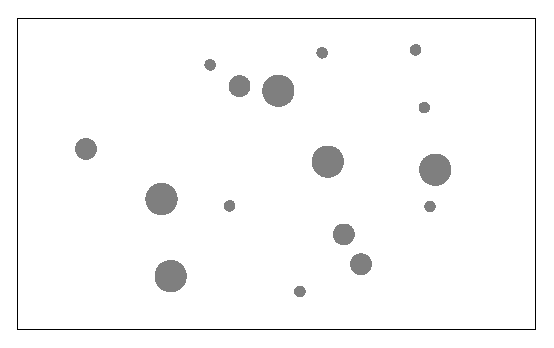
\includegraphics[width=0.3\textwidth,height=!]{nuclei}
\end{figure}

\smallskip \subp
Assume all nuclei are spherical.
Each nucleus contains $m = 1,2,3,\ldots$ molecules.
The free energy of each nucleus consists of a bulk
and a surface energy term.
Each molecule contributes $-\delta$ to free energy
when forming a nucleus.
The interfacial tension between a nucleus 
and its surroundings is a constant $+\gamma$.
Show that the free energy of a nucleus
with $m$ molecules is:
\[ g_m = \tilde\gamma\, m^{2/3} - \delta\, m, \]
where $\tilde\gamma = \gamma (36\pi v_0^2)^{1/3}$,
and $v_0$ is the volume of one molecule.
\solution{\\
We can write the free energy as $g_m = -\delta m + \gamma A$.
Since the nuclei are spherical, 
\[ V = m v_0 = \frac{4}{3}\pi R^3 \quad \Rightarrow \quad
   R = \left( \frac{3 m v_0}{4\pi} \right)^{1/3} \]
\[ A = 4 \pi R^2 = (64 \pi^3)^{1/3} 
       \left( \frac{9 m^2 v_0^2}{16 \pi^2} \right)^{1/3} 
     = \left( 36 \pi v_0^2\right)^{1/3} m^{2/3} \]
Clearly, 
$\gamma A = \gamma (36 \pi v_0^2)^{1/3} m^{2/3} = \tilde{\gamma} m^{2/3}$. 
\[ \boxed{ g_m = \gamma A - \delta m = \tilde{\gamma} m^{2/3} - \delta m } \]
}

\smallskip \subp
Treat the multi-nuclei system as an ideal gas
at temperature $T$.
Let the system volume be $V$,
and the number of nuclei of size $m$ be $n_m$.
Show that the total free energy is given by
$$
F = \sum_{m=1}^\infty n_m \left[ g_m 
    - \kT \ln\left(\frac{V e}{n_m \Lambda_m^3} \right) \right].
$$
Here $\Lambda_m$ is the thermal de~Broglie wavelength
for the nucleus of size $m$.
\solution{\\
Begin by writing the single-particle partition function
for a nucleus with $m$ molecules, $q_m$. 
\[ q_m = q_{\rm tr} q_{\rm int} = \left( \frac{V}{\Lambda_m^3} \right) 
                                  \exp \left( -\frac{g_m}{\kT} \right) \]
Assuming the nuclei do not interact with each other (i.e. ideal gas),
we know from class that $q_{\rm tr} = V/\Lambda_m^3$. 
What about the internal degrees of freedom?
Recall that free energy is related to partition function as 
$F = -\kT \ln Q$. Naturally, we conclude that the
free energy in part (a) must account for internal degrees of freedom:
\[ g_m = -\kT \ln q_{\rm int} \quad \Rightarrow \quad 
   q_{\rm int} = \exp \left( -\frac{g_m}{\kT} \right) \]
Nuclei of the same size should be indistinguishable. 
The partition function for a non-interacting system
of polydisperse (different sizes) particles is given by:
\[ Q = \prod_m^\infty \frac{q_m^{n_m}}{n_m!} 
     = \prod_m^\infty \frac{1}{n_m!} \left( \frac{V}{\Lambda_m^3} \right)^{n_m} 
       \exp \left( \frac{-n_m g_m}{\kT} \right) \]
We know the Helmholtz free energy is $F = \kT \ln Q$, as usual:
\begin{align*}
   F &= -\kT \ln Q 
      = -\kT \sum_m^\infty \left[ -n_m \ln \left( \frac{n_m}{e} \right) 
      + n_m \ln \left( \frac{V}{\Lambda_m^3} \right) - \frac{n_m g_m}{\kT} \right] \\
     &= \sum_m^\infty n_m \left[ -\kT \ln \left(\frac{Ve}{n_m \Lambda_m^3} \right) 
      + g_m \right]
\end{align*}
\[ \boxed{ F = \sum_{m=1}^\infty n_m \left[ g_m 
             - \kT \ln \left( \frac{V e}{n_m \Lambda_m^3} \right) \right] } \]
}

\smallskip \subp
The total number of molecules in the system is conserved.
Therefore, $N = \sum_{m = 1}^\infty n_m \,m $ must be constant.
Show that minimizing total free energy $F$
subject to this constraint yields the following
expression for the optimal value of $n_m$,
where $\phi_m \equiv n_m \Lambda_m^3 / V$ is the volume fraction.
\[ \phi_m = \phi_1^m \exp\left(-\frac{g_m - m g_1}{\kT}\right) . \]
Above, $\phi_1$ and $g_1$ are the volume fraction
and free energy of a unimer ($m=1$).
\solution{\\
We incorporate the constraint using the Lagrange multiplier, $\lambda$.
\begin{align*}
   \frac{\partial}{\partial n_m} 
  &\left[ \sum_{j=1}^\infty \left( n_j g_j 
        - n_j \kT \ln \left( \frac{Ve}{n_j \Lambda_j^3}\right) \right) 
        - \lambda \left( \sum_{j=1}^\infty j n_j - N \right) \right] \\
= &\left[ g_m - \kT \ln \left( \frac{Ve}{n_m \Lambda_m^3} \right)
        - n_m \kT \left(- \frac{1}{n_m} \right) - m\lambda \right] \\
= &\,\, \kT \left[ \frac{g_m}{\kT} - \ln \left( \frac{V}{n_m \Lambda_m^3} \right)
            - \ln(e) + 1 \right] - m \lambda \\
= &\,\, \kT \left[ \frac{g_m}{\kT} + \ln \phi_m \right] - m \lambda = 0
\end{align*}
Rearrange to solve for $\phi_m$, 
and use $\phi_1$ as a reference to solve for $\lambda$.
\[ \ln \phi_m = \frac{m \lambda - g_m}{\kT} \quad \Rightarrow \quad 
   \phi_m = \exp \left( - \frac{g_m - m \lambda}{\kT} \right) \]
\[ \phi_1 = \exp \left( - \frac{g_1 - \lambda}{\kT} \right) \quad \Rightarrow \quad
   \lambda = g_1 + \kT \ln \phi_1 \]
Substitute this back into $\phi_m$:
\[ \phi_m = \exp \left( -\frac{g_m}{\kT} \right) 
            \exp \left( \frac{m g_1 + m \kT \ln \phi_1}{\kT} \right) 
          = \exp \left( -\frac{g_m}{\kT} \right) 
            \exp \left( \frac{m g_1}{\kT} \right) 
            \exp \left( m \ln \phi_1 \right) \]
Since $m \ln \phi_1 = \ln \phi_1^m$, we are done:
\[ \boxed{ \phi_m = \phi_1^m \exp \left( -\frac{g_m - m g_1}{\kT} \right) } \]
\newpage
}

\smallskip \subp
Sketch, qualitatively, how the volume fraction $\phi_m$ varies with $m$.
Show that $\phi_m$ has an extreme value (maximum or minimum),
and that the corresponding critical nucleus size is given by
$$
m^* = \left[ \frac{3}{2} \left(1 +
  \frac{\kT}{\tilde\gamma} \ln\phi_1\right) \right]^{-3} .
$$
Note that the minimum unimer concentration needed for nucleation is
$ \phi_{1,\rm min} = e^{-\tilde\gamma/(\kT)} $.
\solution{\\
Substitute in $g_m$ as derived in part (a):
\[ g_m - m g_1 = \tilde{\gamma} m^{2/3} - \delta m - m (\tilde{\gamma} - \delta) 
               = \tilde{\gamma} (m^{2/3} - m) \]
It is more convenient to absorb the leading $\phi_1^m$ back into the exponential:
\[ \phi_m = \phi_1^m \exp \left( -\frac{g_m - m g_1}{\kT} \right) 
          = \exp \left[ -\frac{\tilde{\gamma}}{\kT} (m^{2/3}-m) 
                        +m \ln \phi_1 \right] \]
The extremum of an exponential is the same as 
the extremum of its argument.
\[ \frac{\partial}{\partial m} 
   \left[ -\frac{\tilde{\gamma}}{\kT} (m^{2/3}-m) + m \ln \phi_1 \right] 
 = -\frac{\tilde{\gamma}}{\kT} \left( \frac{2}{3m^{1/3}} - 1 \right) + \ln \phi_1 
 = 0\]
Solve the expression above for $m$:
\[ \frac{2}{3m^{1/3}} = 1 + \frac{\kT}{\tilde{\gamma}} \ln \phi_1 
   \quad \Rightarrow \quad
   m^{-1/3} = \frac{3}{2} \left( 1 + 
             \frac{\kT}{\tilde{\gamma}} \ln \phi_1 \right) \]
\[ \boxed{ m^* = \left[ \frac{3}{2} \left( 1 + 
               \frac{\kT}{\tilde{\gamma}} \ln \phi_1 \right) \right]^{-3} } \]
We should check if $m^*$ corresponds to a maximum or a minimum.
\[ \frac{\partial^2 \phi_m}{\partial m^2}
 =  \frac{\partial}{\partial m} 
    \left[ - \frac{\tilde{\gamma}}{\kT} \left( \frac{2}{3m^{1/3}} - 1 \right)
           + \ln \phi_1 \right] 
 = -\frac{\tilde{\gamma}}{\kT} \left[ -\frac{2}{9m^{4/3}} \right] 
 = \frac{2\tilde{\gamma}}{9 \kT m^{4/3}} > 0 \]
This indicates that $m^*$ corresponds to a minimum.
In nucleation theory, when $m < m^*$, the nucleus is unstable
and will shrink until it ceases to exist.
If a nucleus grows to $m > m^*$, the favorable
nucleus-forming free energy overtakes surface tension
and the nucleus will continue to grow.
Therefore, it makes sense that $m^*$ corresponds to minimum 
$\phi_m$, as the energetics of this system dictate that
nuclei will be driven towards either $m=0$ or $m\to\infty$.
For points, $\phi_m$ should be concave up with respect to $m$. 
The actual function is plotted below.
\begin{figure}[h]\centering
\includegraphics[width=0.55\textwidth,height=!]{nucleationphi}
\end{figure}
\newpage
}

\bigskip \problem2
{\bf Bonus}:
The word {\sl entropy} was invented by which scientist?
\solution{\\ Rudolf Clausius.}